% !TeX root = ../main.tex

\addcontentsline{toc}{chapter}{\appendixPhrase}
\chapter{Experiment 1 - Verlustkurven}
\label{appendix:Experiment1Verlustkurven}
\begin{figure}[ht]
	\centering
	\begin{subfigure}[b]{0.8\textwidth}
		\centering
		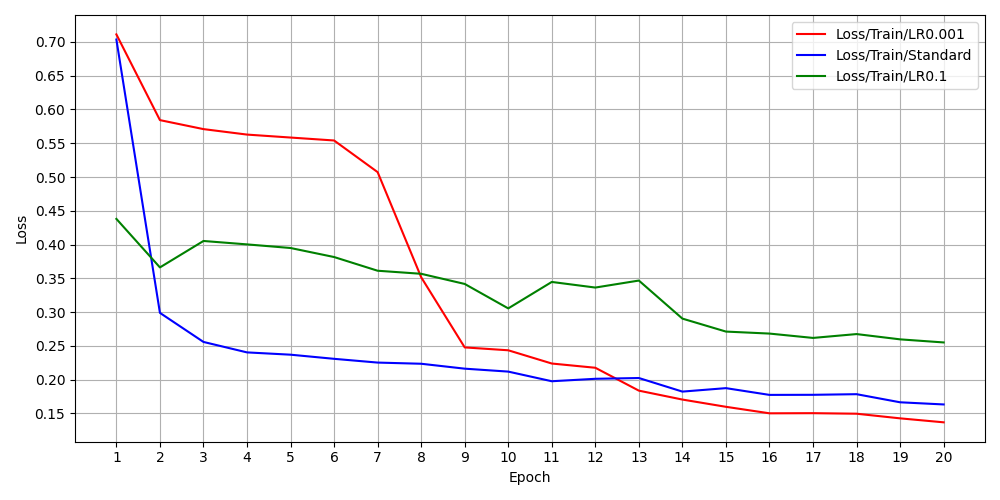
\includegraphics[width=\linewidth]{LR_experiment_train.png}
		\caption{Trainingsverlust}
		\label{fig:ex1_lr_train}
	\end{subfigure}
	\vfil
	\begin{subfigure}[b]{0.8\linewidth}
		\centering
		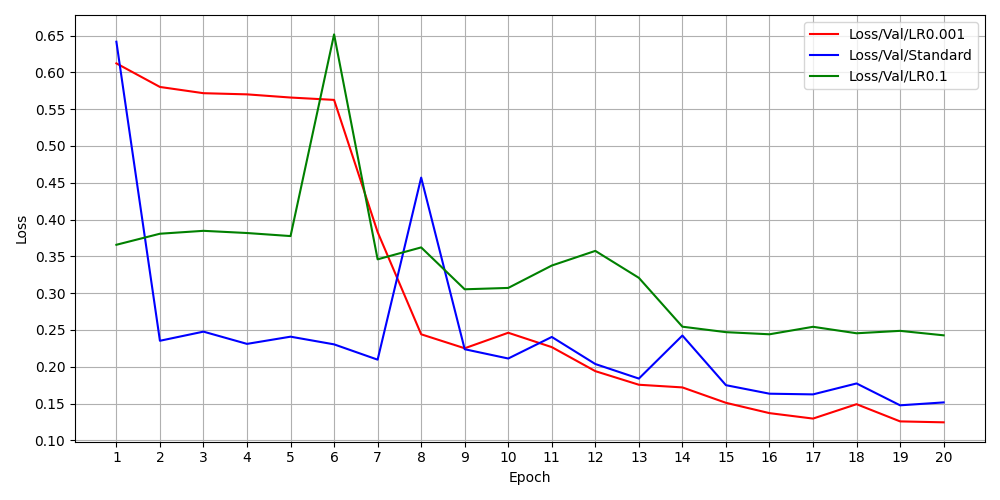
\includegraphics[width=\textwidth]{LR_experiment_val.png}
		\caption{Validierungsverlust}
		\label{fig:ex1_lr_val}
	\end{subfigure}
	\caption{Experiment 1 - Verlustkurven von Training und Validierung über 20 Epochen, mit den Lernraten $0.1$, $0.01$(Standard) und $0.001$ (Quelle: Eigene Darstellung)}
\end{figure} 

\chapter{Experiment 2 - Verlustkurven}
\label{appendix:Experiment2Verlustkurven}
\begin{figure}[ht]
	\centering
	\begin{subfigure}[b]{0.8\textwidth}
		\centering
		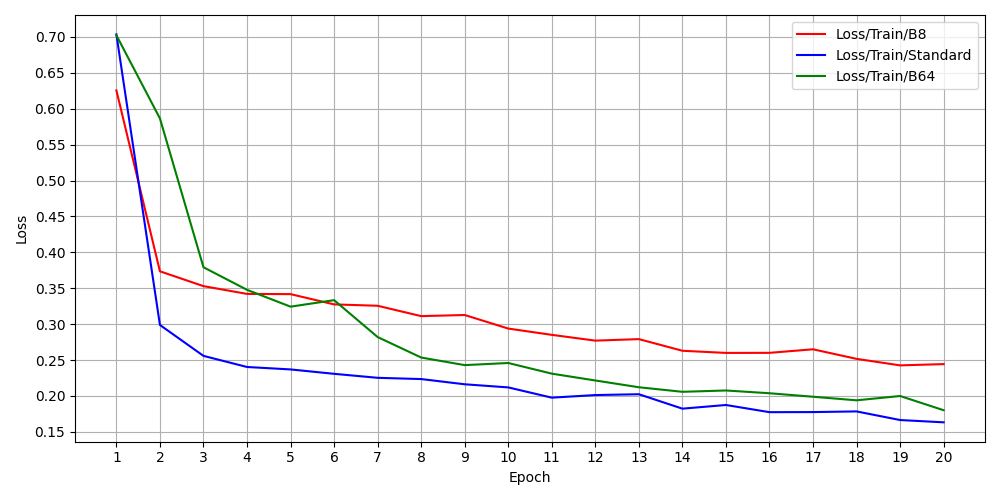
\includegraphics[width=\linewidth]{Batch_experiment_train.png}
		\caption{Trainingsverlust}
		\label{fig:ex2_batch_train}
	\end{subfigure}
	\vfil
	\begin{subfigure}[b]{0.8\linewidth}
		\centering
		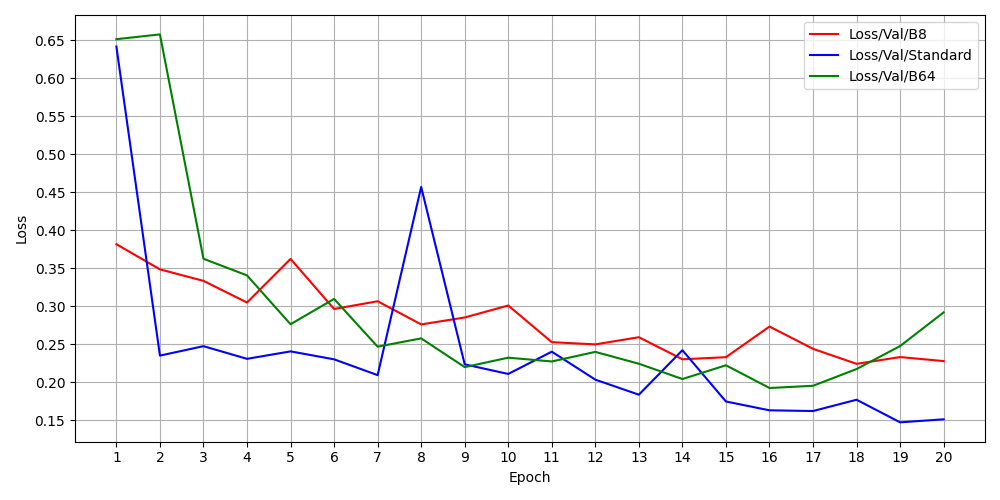
\includegraphics[width=\textwidth]{Batch_experiment_val.png}
		\caption{Validierungsverlust}
		\label{fig:ex2_batch_val}
	\end{subfigure}
	\caption{Experiment 2 - Verlustkurven von Training und Validierung über 20 Epochen, mit den Batch Größen $8$, $32$(Standard) und $64$ (Quelle: Eigene Darstellung)}
\end{figure} 

\chapter{Experiment 3 - Verlustkurven}
\label{appendix:Experiment3Verlustkurven}
\begin{figure}[!ht]
	\centering
	\begin{subfigure}[b]{0.8\textwidth}
		\centering
		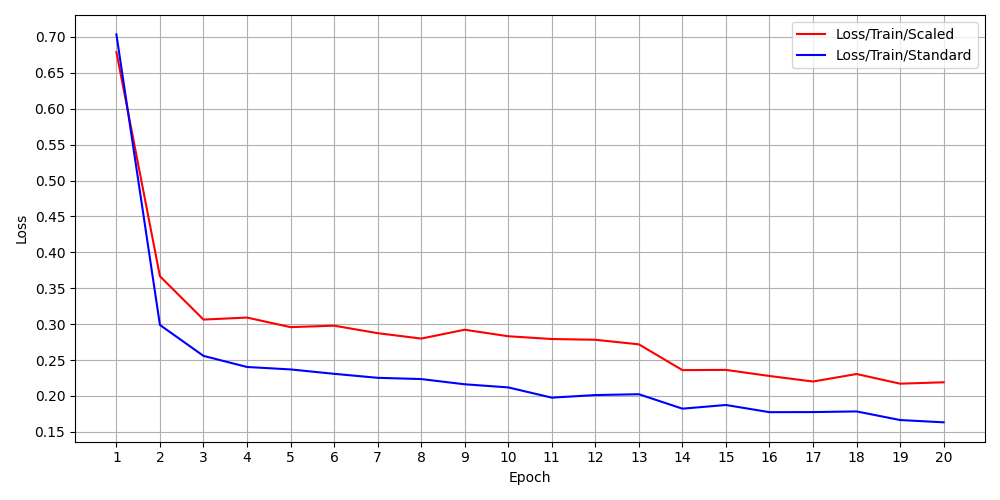
\includegraphics[width=\linewidth]{Prepro_experiment_train.png}
		\caption{Trainingsverlust}
		\label{fig:ex3_prepro_train}
	\end{subfigure}
	\vfil
	\begin{subfigure}[b]{0.8\linewidth}
		\centering
		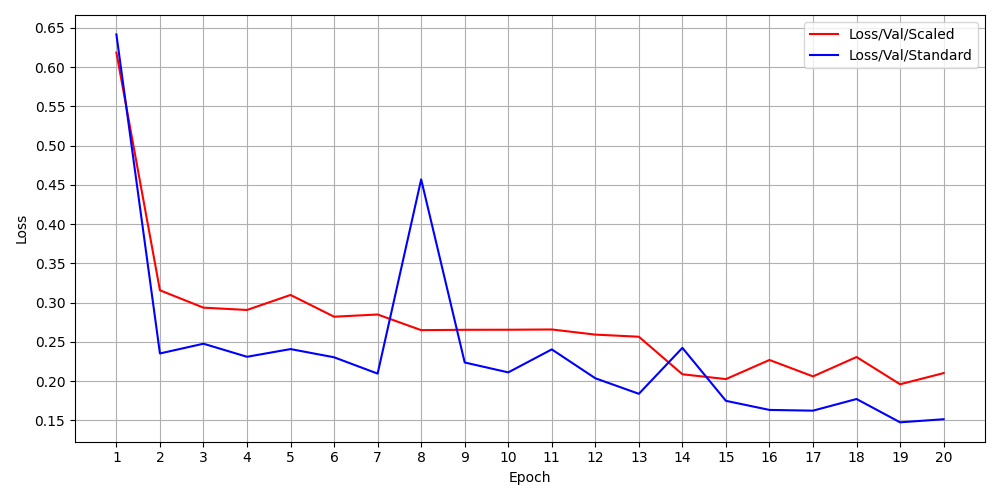
\includegraphics[width=\textwidth]{Prepro_experiment_val.png}
		\caption{Validierungsverlust}
		\label{fig:ex3_prepro_val}
	\end{subfigure}
	\caption{Experiment 3 - Verlustkurven von Training und Validierung über 20 Epochen, mit je Zuschneiden (Standard) und Größenskalierung (Scaled) (Quelle: Eigene Darstellung)}
\end{figure} 